\documentclass{scrartcl}
\usepackage[utf8]{inputenc}
\usepackage[colorlinks=true,urlcolor=black,linkcolor=black]{hyperref}
\usepackage{graphicx}
\title{Projet Discret\\Rapport Pédagogique}
\author{Thomas BENOIT,\\Zied BEN OTHMANE, Adrien BISUTTI, Lydie RICHAUME}
\date{Mars 2016}

\begin{document}

\maketitle

\tableofcontents
\newpage

%----------------------------------------------------------
%INTRODUCTION
%----------------------------------------------------------

\section{Introduction}

%Contexte------------------------------
\subsection{Contexte}
\paragraph{}
Dans le cadre de notre formation de deuxième année de master d'informatique nous avons eu à réaliser un projet à destination de clients réels. Ce projet s'est déroulé sur six mois\,: depuis Octobre jusqu'en Mars. Il permet de mettre en pratique les compétences que nous avons acquises durant nos cours de gestion de projet, ainsi que de nous confronter au développement d'un projet de dimension moyenne.

\paragraph{}
Nos clients, \'Eric Andres et Gaëlle Largeteau-Skapin, ont développé un algorithme de génération de surfaces de révolution discrètes et souhaitaient pouvoir mettre à disposition un outil qui permettrait d'étayer leur publication.

\paragraph{}
Une surface de révolution est un objet mathématique en trois dimensions généré à l'aide de deux courbes en deux dimensions\,: la courbe de révolution et la méridienne. La courbe de révolution (le plus souvent un cercle) définit la transformation à appliquer à la méridienne afin de générer la surface de révolution.

%Problématique-------------------------
\subsection{Problématique}
\paragraph{}
Le but de ce projet est de construire un site web qui permette de créer une surface de révolution discrète à partir d'une courbe dessinée à main levée ou décrite à partir d'une équation. Ce site doit aussi permettre de modifier la courbe de révolution et d'exporter les surfaces obtenues ainsi que de les examiner coupe par coupe.

%Travail réalisé-----------------------
\subsection{Travail réalisé}
\paragraph{}
Afin de répondre à cette problématique, nous avons réalisé une application web se basant sur les technologies HTML5/CSS, Javascript et WebGL qui respecte le cahier des charges\footnote{Présent en annexe.} signé par les clients.
\paragraph{}
\begin{center}
Screen de l'application
\end{center}
\paragraph{}
Le travail réalisé comprend également une documentation technique (architecture de l'application sous forme de diagrammes de classes et documentation du code générée avec JSDoc) qui permet de maintenir et de faire évoluer l'application.

%Organisation du rapport---------------
\subsection{Organisation du rapport}
\paragraph{}
\newpage

%----------------------------------------------------------
%TRAVAIL REALISE
%----------------------------------------------------------

\section{Travail réalisé}
\paragraph{}
Dans cette section nous décrirons les fonctionnalités développées en lien avec le cahier des charges. Nous détaillerons les difficultés que nous avons pu rencontré ainsi que les solutions que nous avons mises en place.

%HTML et CSS--------------------------
\subsection{HTML et CSS}
\paragraph{}

%Fonctionnalités----------------------
\subsection{Fonctionnalités}
\paragraph{}

%3D-----------------------------------
\subsubsection{3D}
\paragraph{}

%2D-----------------------------------
\subsubsection{2D}
\paragraph{}

%Gestion de données-------------------
\subsubsection{Gestion de données}
\paragraph{}

%Traduction---------------------------
\subsubsection{Traduction} %Supprimer ?
\paragraph{}

\newpage

%----------------------------------------------------------
%CONDUITE DE PROJET
%----------------------------------------------------------

\section{Conduite de projet}

%Rôles--------------------------------
\subsection{Rôles}
\paragraph{}
Notre équipe est composée de quatre personnes\,: 
\begin{itemize}
    \item Thomas Benoît - Chef de projet
    \item Zied Ben Othmane - Responsable qualité
    \item Adrien Bisutti - Responsable des risques
    \item Lydie Richaume - Responsable des tâches
\end{itemize}

%Méthode de développement-------------
\subsection{Méthode de développement}
\paragraph{}
Nous avons choisi un cycle de développement en spirale. En effet, cela nous permettait de travailler de manière incrémentale et de garder un contact constant avec les clients afin d'être certains de leur satisfaction, tout en gardant une certaine souplesse quant à la durée de chaque cycle.

%Planification------------------------
\subsection{Planification}
\paragraph{}


%Gestion des risques------------------
\subsection{Gestion des risques}
\paragraph{}
Nous avons identifié une vingtaine de risque, les plus importants, dont les fiches sont fournies en annexe, étant\,: 
\begin{itemize}
    \item la possibilité d'un nouveau client\,;
    \item la possibilité d'une évolution de l'algorithme fourni par le client\,;
    \item la possibilité que le rendu 3D demande trop de ressources\,;
    \item 
\end{itemize}

\paragraph{}
Nous avons été prévenus dès le début du projet que celui-ci avait été proposé comme projet transdisciplinaire au sein de l'université. Cela pouvait se traduire par un ajout de clients menant possiblement à une modification du cahier des charges. Cela aurait donc pu impacter fortement notre projet, notamment au niveau des délais\,: en effet, la conception réalisée en début de projet aurait pu ne plus convenir et nous aurions pu avoir à modifier des fonctionnalités déjà développées.

Afin de pouvoir anticiper ces problèmes, il a été décidé que nous demandions un maximum d'informations concernant les changements potentiels à nos clients et que nous nous tenions régulièrement informé des évolutions du dossier.

Ce risque s'est avéré (date)\,: le projet de l'université a été accepté et nos clients ont assisté à une réunion avec les nouveaux clients. Il en est rapidement ressorti que l'université n'aurait pas de demandes supplémentaires. Le degré de gravité du risque a donc diminué.

\paragraph{}
Il a été annoncé dès le début du projet que nos clients travaillaient encore sur de nouvelles versions de leur algorithme. Il était donc possible que nous ayons a inclure des fonctionnalités supplémentaires à celles spécifiées au départ du projet. Cela pouvait donc impacter nos délais par l'ajout de tâches résultant. 

Afin d'éviter que cela nous fasse prendre un retard trop grand, il a été décidé que nous n'accepterions pas de modifications annoncées moins d'un mois avant la fin du projet, et que nous nous informerions régulièrement auprès des clients de l'avancement de leurs recherches afin d'anticiper toute modification de planning.

Ce risque ne s'est finalement pas avéré.

\paragraph{}
Notre projet reprenait le squelette d'un projet précédent et un problème connu était la lenteur du rendu 3D lors de l'affichage d'une quantité trop importante de voxels. Cela pouvait donc avoir un impact important sur les performances de l'application. Afin de palier ce problème, nous avons prévu une tâche visant à améliorer l'algorithme de génération.

Cette tâche a effectivement permis d'obtenir un temps de rendu acceptable sur la plupart des machines, mais le temps de rendu peut rester long lorsque l'on choisit les dimensions maximales pour l'espace 3D.

\paragraph{}
Bien que nous développions une application web, nous n'avons pas eu à gérer les risques liés à l'utilisation d'un serveur. En effet, notre projet était développé uniquement en HTML et Javascript, et il était mentionné dans le cahier des charges que l'hébergement de l'application serait laissé à la charge du client.

%Plan qualité logiciel----------------
\subsection{Plan qualité logicielle}
\subsubsection{La norme ISO 9126}
Nous avons mesuré la qualité logicielle en se basant sur la norme ISO 9126 qui est une norme standard internationale visant à évaluer
la qualité logicielle. Elle normalise et classifie un certain nombre de principes qualité.Elle est composée de six caractéristiques générales qui définissent la qualité globale d'une application : la capacité fonctionnelle, la fiabilité, l'efficacité, la maintenabilité, la facilité d'usage, la portabilité. Chacune de ces caractéristiques est décomposée en sous caractéristiques.
Cette norme semble être une bonne approche pour déterminer la qualité de notre logiciel dans son ensemble et fournir une vue globale satisfaisante.

 \begin{center}
 	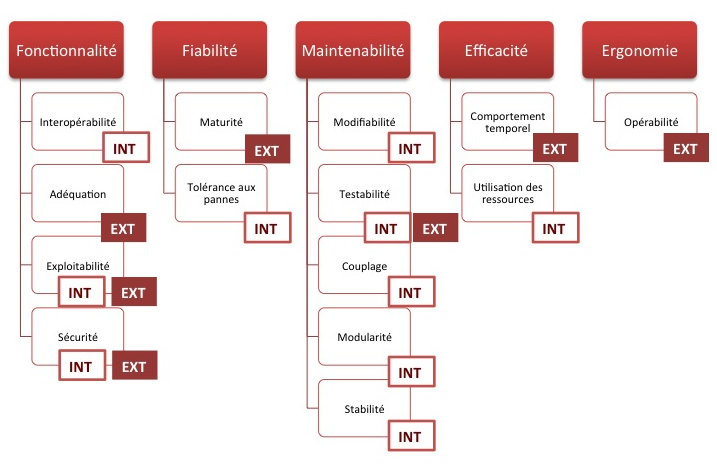
\includegraphics[width=0.60\columnwidth]{iso9126}
 	\captionof{figure}{Résumé des attributs qualité ISO 9126}
 	\label{fig-label}
 \end{center}
\subsubsection{Démarche générale}
Pour mesurer la qualité de notre logiciel nous avons commencer par déterminer son adéquation par rapport aux objectifs de départ et aux standards de programmation. Nous avons ensuite définir précisément ce que l’application doit faire et comment elle doit le faire, tant d’un point de vue fonctionnel que d’un point de vue technique. Aprés avoir fixé ces objectifs,nous avons appliquer un ensemble de règles et de mesures afin de calculer la différence entre objectifs attendus et réalisation obtenue .
 
\subsubsection{Les métriques de mesure}
Pour fournir une représentation de la qualité à un niveau élevé, Nous somme basé sur le modèle ISO 9126 qui s'appuie sur des métriques,Nous avons utilisé un nombre considérable de métriques et certaines d’entre elles ne sont pas calculées de la même manière selon le critère ou le sous-critère à mesurer. Toute les métriques sont été définit et leurs calcul est bien expliqué dans le plan qualité logicielle .
\subsubsection{Résultats obtenus}

Nous avons générer des modèles statistique pour mettre en évidence toute les mesures de la qualité des différentes version de notre application, ces modèles fournit des indications précises sur l'utilisation et l'évaluation du qualité logicielle. Il s'agit de donner du sens en terme à des informations brutes dont l'explication de l'évaluation des résultats sera dans la sous section suivante.

 \begin{center}
 	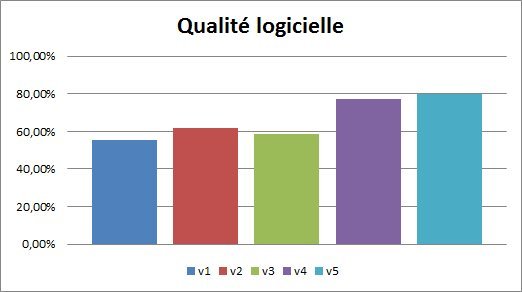
\includegraphics[width=0.60\columnwidth]{evalqualit}
 	\captionof{figure}{Evolution de la qualité logicielle}
 	\label{fig-label}
 \end{center}

  \begin{center}
  	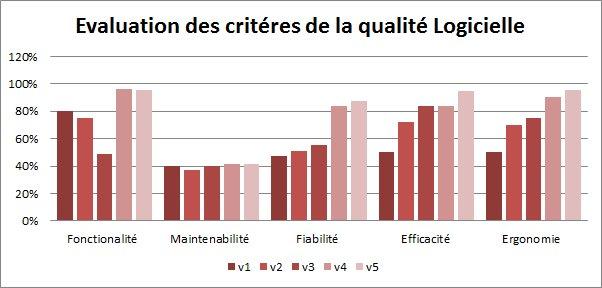
\includegraphics[width=0.60\columnwidth]{cirqualit}
  	\captionof{figure}{Résumé des critères de la qualité logicielle}
  	\label{fig-label}
  \end{center}
\subsubsection{Évaluation des résultats}
Nous identifions six principes fondamentaux pour évaluer notre travail en suivant les indicateurs de qualité de la norme ISO 9126, ces principes sont illustrés dans la mesure des critères de la norme dans les détails sont été expliqué dans le rapport PAQL:

\begin{enumerate}
	\item la capacité fonctionnelle:
C'est-à-dire la capacité qu'ont les fonctionnalités d'un logiciel à répondre aux exigences et besoins explicites ou implicites des usagers.
	\item la facilité d'utilisation :
qui porte sur l'effort nécessaire pour apprendre à manipuler le logiciel.
	\item la fiabilité:
c'est-à-dire la capacité d'un logiciel de rendre des résultats corrects quelles que soient les conditions d'exploitation.
	\item la performance:
c'est-à-dire le rapport entre la quantité de ressources utilisées (moyens matériels, temps, personnel), et la quantité de résultats délivrés.
	\item la maintenabilité
qui mesure l'effort nécessaire à corriger ou transformer le logiciel.
	\item la portabilité:
c'est-à-dire l'aptitude d'un logiciel de fonctionner dans un environnement matériel ou logiciel différent de son environnement initial.
\end{enumerate}

%Coûts--------------------------------
\subsection{Coûts}
\paragraph{}

\newpage

%----------------------------------------------------------
%CONCLUSION
%----------------------------------------------------------

\section{Conclusion}
\paragraph{}

\newpage

%----------------------------------------------------------
%ANNEXE
%----------------------------------------------------------

\section{Annexes}

\end{document}
